\section{Introduction}

% Skim 5/15/07
We introduce a Matlab package, SparsePOP for finding global optimal solutions of polynomial
optimization problems (POPs). An important feature of SparsePOP is ability to
exploit the sparsity of POPs in a way that it can handle  POPs of larger dimensions.
The package is an implementation
of a sparse semidefinite programming (SDP) relaxation method for POPs  in  \cite{WAKI04}, proposed
to improve
the efficiency of  Lasserre's hierarchy of LMI relaxations of increasing dimensions 
\cite{LAS01}. 
See also \cite{KIM03,KOJ03a}. 

 
% Skim 5/15/07
We briefly describe a general POP. 
Let $\Real^n$ and $\Integer^n_+$  denote the $n$-dimensional
Euclidean space and the set of nonnegative integer vectors in $\Real^n$, respectively. 
A real-valued polynomial $f_k(\x)$ 
in $\x =(x_1,x_2,\ldots,x_n) \in \Real^n$ is expressed as
\[
	\begin{array}{lllll}
     f_k(\x) & = \displaystyle \sum_{\balpha \in \FC_k} c_k(\balpha) \x^{\salpha},\ \x \in \Real^n,   \
	 c_k(\balpha)  & \in \Real, \ 
	\FC_k  \subset \Integer_+^n
	\end{array}
\]
$(k=0,1,2,\ldots,m)$, where      
$\displaystyle \x^{\salpha} = x_1^{\alpha_1}x_2^{\alpha_2} \cdots
x_n^{\alpha_n}$ for every $\x =(x_1,x_2,\ldots,x_n) \in \Real^n$ and 
every $\balpha \in \Integer^n_+$.
% Skim 5/15/07 
We consider a POP in the following form: 
\begin{equation}
\left.
\begin{array}{llll}
\mbox{minimize } & f_0(\x) \\
\mbox{subject to } & f_k (\x) \geq 0 & (k=1,2,\ldots,\ell), \\
                                 & f_k(\x) = 0 & (k=\ell+1,\ldots,m), \\
                                 & \mbox{lbd}_i \leq x_i \leq \mbox{ubd}_i & (i=1,2,\ldots,n), 
\end{array}
\right\} \label{POP0}
\end{equation}
where $-\infty \leq  \mbox{lbd}_i < \infty$ and $-\infty <  \mbox{ubd}_i \leq \infty$ $(i=1,2,\ldots,n)$. 
Let $\zeta^*$ denote the optimal value of the POP (\ref{POP0}). 

The package accepts a POP as input, and outputs 
solution information and statistics. The main part 
constructs a sparse SDP relaxation  of  the POP  and uses
SeDuMi \cite{STRUM99} to obtain an approximate global optimal solution.
The structure of the software package SparsePOP is shown in Figure \ref{structure}. 
% Skim 5/15/07
The function sparsePOP.m is the main function of SparsePOP. 
Note the difference in the names of the function sparsePOP.m and 
%while the package name is the SparsePOP.
the package SparsePOP.
As %will be seen
will be shown in Section~\ref{Representation},
sparsePOP.m accepts two different formats of a POP:
the \GMS format \cite{GAMS} that is more readable,
and  the SparsePOP format, a set of 
MATLAB data types designed exclusively for SparsePOP. If a POP is read in the \GMS format, 
then a subfunction readGMS.m %of the sparsePOP.m
 converts a \GMS format of the POP 
to a sparsePOP format of the POP.  It is followed by checking the validity  of 
the SparsePOP format of the POP and the parameters optionally 
provided by the user or given by default.  Then, either SDPrelaxation.m or SDPrelaxationMex.m 
transforms the POP into an SDP relaxation problem, and solves it with a MATLAB SDP solver 
SeDuMi. Once the POP (\ref{POP0}) is solved, 
the solution information is written using the MATLAB function printSolution.m. We refer to the paper 
\cite{WAKI04} for numerical results from SparsePOP. 

% Skimm 5/15/07
The conversion from a POP to an SDP relaxation problem can be time-consuming if implemented
with MATLAB. The subfunction SDPrelaxationMex.m is developed in C++ to speed up this process.
SparsePOP provides an option of choosing SDPrelaxation.m or SDPrelaxationMex.m.
If   the C++ source programs can be compiled and linked
into mex files,  the SDPrelaxationMex.m is recommended.  Otherwise, %user needs to change 
the value of the parameter {\sf param.mex} should be changed
from {\sf param.mex = 1} to {\sf param.mex = 0} in the defaultParameter.m to choose the 
SDPrelaxation.m.
 
\begin{figure}
\label{structure}
\begin{center}
% \hspace{-1cm}
\epsfig{file=system.eps,height=9cm}
\caption{The structure of the main function sparsePOP.m}
\end{center}
\end{figure}
 
 % Skim 5/15/07
This paper is organized as follows:
In Section~\ref{sec:csp}, we give a brief introduction of the 
sparse SDP relaxation % of Waki, Kim, Kojima and Muramatsu 
\cite{WAKI04} for POPs. Section 3 includes the description of 
%Then we explain
two formats to express polynomials and POPs. %in Section~\ref{Representation}.
Exemplary execution is shown in Section~\ref{sample}. %presents execution examples of our software, and 
Section~\ref{multiple} contains the discussion of
how  POPs having possibly  multiple optimal solutions can be treated. 
%Section  includes details of output of 
The main  function 
sparsePOP.m and its  subfunctions readGMS.m, SDPrelaxation.m, SDPrelaxationMex.m 
and printSolution.m shown in Figure~\ref{structure} are described with their
input and output arguments in Section~\ref{mainFunctions}. 
%Section~\ref{PARAM} is devoted to explain 
The parameters %that are passed 
to the subfunctions SDPrelaxation.m and SDPrelaxationMex.m
are explained in Section~\ref{PARAM}.
